\documentclass{memoir}
\usepackage{hyperref}
\usepackage{graphicx}
\graphicspath{ {figures/} }

\title{Distributed Systems:\\Crossing Intersection with Autonomous Vehicles}

\author{Antonio Toncetti\\Gabriele Venturato\\\\DMIF, University of Udine, Italy}

\date{%Version 0.1, 
	\today}

\begin{document}


%\begin{titlingpage}
\maketitle
\begin{abstract}
The aim of this project is to provide an implemented solution to the problem of autonomous vehicles crossing an intersection.
Although the solution relies on some simplifications, it can be further elaborated to work in a real-case scenario.

The solution proposed in this report is meant to be more general and as modular as possible, in order for it to be possibly extended in a concrete situation.
\end{abstract}
%\end{titlingpage}

\chapter{Introduction}\label{ch:intro}

The problem to solve is the one in which some autonomous vehicles have to cross an intersection without being involved in road accidents. 

The idea is to solve the problem for a generic intersection. The autonomous vehicles can't rely on a central server, they have to cooperate with each other to cross the intersection by taking decisions which ensure a \emph{fair} and \emph{safe} policy. In particular there are two components in the proposed solution: vehicles and the environment. The latter is necessary in this context in order to simulate sensors that are usually inside autonomous vehicles which allows them to interact with the environment (e.g. proximity sensors, GPS, cameras, etc\dots).
The system is \emph{fault tolerant}, but neither byzantine processes nor cybersecurity hazards are taken in consideration, for simplification purpose.

The report starts by analysing the project: Chapter~\ref{ch:analysis} is devoted to functional and non-functional requirements, and system assumptions too. Chapter~\ref{ch:project} contains the description of the general architecture, and specific algorithms.

Following chapters aim to describe details of the implementation, and validation w.r.t. requirements.



\chapter{Analysis}\label{ch:analysis}

This chapter describes in detail some fundamental assumptions about the system, as well as functional and non-functional requirements.

\section{Assumptions}

Some general considerations are here presented. First of all it's assumed a situation in which each autonomous vehicle knows its destination and the roads it is going to travel, since we can assume that each autonomous vehicle has a GPS device on board.

Moreover it's assumed, for sake of simplicity, that all vehicles have the same dimension --- or better: that each vehicle can fit into a single position of the internal model used to represent the roads. Moreover, common physical quantities (like weight, speed, acceleration, etc\dots) are omitted. Instead, the autonomous vehicles move in unit steps governed by the internal model.
\newline

Further assumptions are:

\begin{itemize}
	\item \emph{Faults}: at any moment a failure can arise in vehicles --- software or mechanical. A mechanical failure doesn't compromise the software abilities, but a software failure implies an hardware failure. Since we can assume that if the software fails, the autonomous vehicle stops and goes in ``emergency mode''. It's also assumed that if a crash happens in queues, there's enough space for the other vehicles to overtake the faulty one; but if the crash happens inside the crossroads it must be managed by removing the faulty vehicle with a tow truck (or something similar).
	\item \emph{Moves}: the path that a vehicle can take inside the interception is predefined and known a priori. From each position there's a unique path to each destination, and no one can modify or choose a different path once decided. A visual representation of this assumption can be found in Figure~\ref{fig:intersection-graph}, in which green dots represent positions occupied while crossing, and light-blue dots are the destinations. Once a vehicle reaches its destination, it is considered ``satisfied'', and can not fail anymore, it can only move forward on its own way. Reversing is not allowed.
\end{itemize}

\begin{figure}
	\centering
	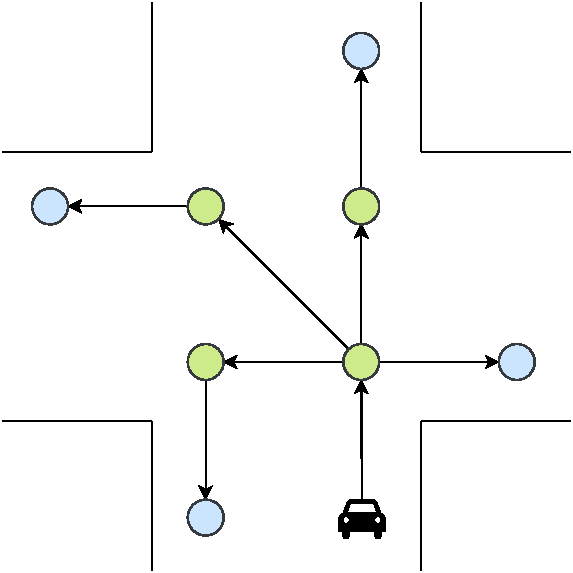
\includegraphics[width=0.4\linewidth]{intersection_graph.pdf}
	\caption{Example of predefined movements that a vehicle can follow in crossing an intersection.}
	\label{fig:intersection-graph}
\end{figure}

\section{Functional requirements}
The solution provides two main modules: \emph{vehicle} and \emph{environment}

\subsection{Vehicle}
Each vehicle has an internal state at any moment. Moreover he:

\begin{itemize}
	\item knows its position and what happens around, through the environment (in a real context this is handled by sensors like GPS and proximity sensors): it can pick up if there are other vehicles trying to cross, or if there is a vehicle in front or behind it;
	\item communicates with its neighbours by sharing: the direction it wants to travel, its internal state, the next position he is about to reach;
	\item if it's in the queue, it knows nothing other than its internal information and that it is taking part in a queue with someone before and possibly behind, it can communicate only with these two;
	\item if it's in the head of the queue, it can connect with other vehicles (that are the head of other queues) that are crossing the intersection;
\end{itemize}

\subsection{Environment}

The environment represent the vehicle's ability to use its sensors. It knows the intersection shape and dimension; it knows vehicles approaching the crossroads and the ones in the queues; it provides vehicles with all the information they need to safely manoeuvre within the environment.

\section{Non functional requirements}
The system doesn't handle byzantine processes nor cybersecurity issues.

\begin{itemize}
	\item \emph{Safeness}: there can't be more than a vehicle in the same position at the same time;
	\item \emph{Liveness}: if a vehicle approaches the intersection and is waiting to cross it, eventually it will cross it;
	\item \emph{Fairness}: if a vehicle approaches the intersection and is waiting to cross it, there exists a bound to the waiting time;
	\item \emph{Fault Tolerant}: the system is tolerant to hardware and software failures;
	\item \emph{Distributed}: there is no central server, vehicles have to coordinate each other.
\end{itemize}



\chapter{Project}\label{ch:project}

The project is developed in \href{https://www.erlang.org/}{Erlang}

\section{Logical architecture}

\section{Protocols and algorithms}

The algorithm described in this section applies to generic intersections. Vehicles queue up along the roads leading to an intersection awaiting for their turn to cross. The first vehicle of a queue is the vehicle at the verge of entering the intersection and we will call such vehicle a participant of the intersection crossing algorithm.

\subsection{Intersection Crossing Algorithm}

The algorithm maintains the following invariant through execution:

\begin{itemize}
	\item one vehicle per time can cross the intersection
	\item only the leader vehicle can cross the intersection
\end{itemize}
Algorithm description:
\begin{enumerate}
	\item The participants (first vehicles in their respective queues) are willing to cross the intersection
	\item They start the Bully Algorithm to elect a leader.
	\item The leader L identifies the next leader by choosing the first vehicle after him in a clockwise manner
	\item The leader begins to cross the intersection
	\item After the leader has successfully crossed the intersection, the lead passes to the chosen vehicle and the algorithm repeats from 3.
\end{enumerate}
Additional details:
\begin{itemize}
	\item After the leader election, every participant knows who is the current leader
	\item Once the leader starts crossing, the vehicle behind him (if any) becomes a new participant and asks to join the algorithm. The other participants answer by providing the identity of the current leader
\end{itemize}
A leader election starts only when one or more vehicles join an empty intersection, i.e. when they become participants and no prior participants are available (the new vehicles don't receive an answer when asking to join the algorithm)

\subsection{Managing abnormal cases}

All participants monitor the leader, if the leader fails, everyone knows who the next leader is (see 3. in the algorithm description).

\begin{itemize}
	\item If the leader fails, the vehicle in clockwise order after him becomes the new leader and the algorithm restarts from 3.
	\item If a participant fails, it is assumed that the next vehicle in the queue becomes a participant.
	\item If a leader fails while crossing, everyone must wait a timeout T for the tow truck to clear the intersection
	\item If the leader undergoes a mechanical failure, it notifies the successful crossing of the intersection (in order to pass the lead to the next vehicle) and requests to be removed. Vehicles in queue behind him must wait for its removal. If the failure happens during the crossing, it notifies the successful crossing only after being removed by the tow truck (?)
\end{itemize}

\section{Physical architecture and deployment}

\section{Development plan}



%\chapter{Implementation}


%\chapter{Validation}


%\chapter{Conclusions}



%\appendix

%\chapter{Appendix}

\end{document}